% https://stackoverflow.com/questions/2801370/how-to-find-intersections-with-ellipses-in-pgf-tikz

\documentclass[border=3pt,tikz]{standalone}
\usepackage{amsmath} % for \dfrac
\usepackage{tikz}
\tikzset{>=latex} % for LaTeX arrow head
\usepackage{pgfplots} % for the axis environment
%\usetikzlibrary{calc} % to do arithmetic with coordinates
%\usetikzlibrary{angles,quotes} % for pic
\pgfplotsset{compat=1.13}
\usetikzlibrary{fadings,intersections}


\begin{document}
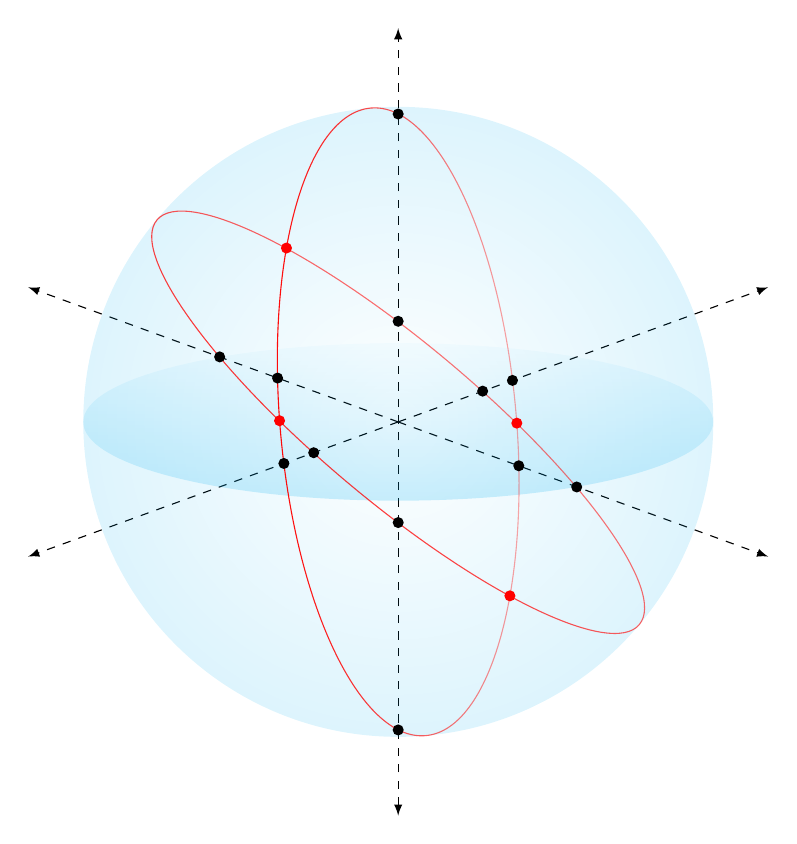
\begin{tikzpicture}
  \tikzfading[ name        = fade right
             , left color  = transparent!20
             , right color = transparent!90 ]

  \tikzfading[name         = fade out
             , inner color = transparent!100
             , outer color = transparent!10 ]

  \tikzfading[name         = fade right gc
             , left color  = transparent!0
             , right color = transparent!70]

  \draw [name path = y  axis, <->, dashed] (0,-5) -- (0,5)   ; % y-axis
  \draw [name path = x- axis,  ->, dashed] (0, 0) -- (20:5)  ; % x-axis
  \draw [name path = x+ axis,  ->, dashed] (0, 0) -- (200:5) ; % x-axis
  \draw [name path = z+ axis,  ->, dashed] (0, 0) -- (340:5) ; % z-axis
  \draw [name path = z- axis,  ->, dashed] (0, 0) -- (160:5) ; % z-axis

  % bounding circle
  \fill [color=cyan, opacity=0.15, path fading=fade out]
        (0,0) circle (4cm) ;

  % x-y-axis area
  \fill [color=cyan, opacity=0.25, path fading=fade right, fading angle=90]
        (0,0) ellipse (4cm and 1cm);

  % great circle 1
  \draw [ name path    = great circle 1
        , rotate       = -40
        , color        = red
        , path fading  = fade right gc
        , fading angle = 40]
        (0,0) ellipse (4cm and 1cm);

  % great circle 2
  \draw [ name path    = great circle 2
        , rotate       = 5
        , color        = red
        , path fading  = fade right gc
        , fading angle = 5]
        (0,0) ellipse (1.5cm and 4cm);

  % Intersections
  \path [name intersections={of=great circle 1 and great circle 2}] ;
  \foreach \i in {1,...,4}
    \fill [color=red] (intersection-\i) circle (2pt) ;

  \path [name intersections={of=y axis and great circle 1}] ;
  \fill (intersection-1) circle (2pt) ;
  \fill (intersection-2) circle (2pt) ;
  \path [name intersections={of=y axis and great circle 2}] ;
  \fill (intersection-1) circle (2pt) ;
  \fill (intersection-2) circle (2pt) ;

  \foreach \a in {x,z} {
    \foreach \ss in {+,-} {
      \def\s.{\ss} % Otherwise the space in `\a\s axis` would get gobbled.
      \path [name intersections={of=\a\s. axis and great circle 1}] ;
      \fill (intersection-1) circle (2pt) ;
      \path [name intersections={of=\a\s. axis and great circle 2}] ;
      \fill (intersection-1) circle (2pt) ;
    }
  }
\end{tikzpicture}
\end{document}
